% Rafael Sartori M. dos Santos, 186154
\documentclass[brazilian,a4paper,twocolumn]{article}

% Título
\title{MC920 -- Trabalho 2}
\author{Rafael Sartori M. Santos, 186154}
\date{1 de outubro de 2019}

% Configuração do documento
\setlength{\parskip}{3pt}
\usepackage[utf8]{inputenc} % tipo de documento UTF-8
\usepackage{mathtools} % permitir expressões matemáticas
\usepackage{breqn} % equações quebradas em várias linhas automaticamente
\usepackage{babel} % configuração da lingua portuguesa
\usepackage{caption} % para legenda de tabelas e figuras
\usepackage[
    pdfauthor={Rafael Sartori M. Santos},
    pdftitle={Trabalho 2 -- MC920},
    pdfproducer={LaTeX (texlive) com hyperref},
    hidelinks
]{hyperref} % para links externos (href)
\usepackage{cleveref} % para referenciar tabelas e figuras melhor
\usepackage{indentfirst} % indentação de todo primeiro parágrafo
\usepackage{graphicx} % para adicionar imagens
\graphicspath{{../imgs_png/}, {../imgs/}} % atalho para o caminho das imagens
\usepackage{float} % para fixar posição de imagens
\usepackage{subcaption} % para imagens ficarem lado a lado
% Usamos geometry pois dá mais espaço que fullpage
%\usepackage{geometry} % alterar geometria do papel
%\geometry{a4paper,left=1.7cm,right=1.7cm,top=1cm,bottom=2.0cm} % menor margem
\usepackage{fullpage} % utilizamos uma versão com menos espaçamento nas bordas
\usepackage{verbatim} % pacote para incluir arquivos em verbatim
\usepackage{mdframed} % para enquadrar coisas

% Início do documento
\begin{document}

\maketitle


\section{Introdução}

    Neste trabalho, temos que avaliar e comparar diferentes métodos de limiarização (locais e globais). Aplicarei cada transformação em imagens monocromáticas em formato PGM fornecidas pelo professor H. Pedrini como sugere o enunciado. O resultado analisarei quanto aos contornos dos objetos, detalhes mantidos da imagem e ruído.

    Executarei esse processamento utilizando Python com as bibliotecas padrão, \href{https://opencv.org/}{\emph{OpenCV}}, \href{https://matplotlib.org/}{\emph{Matplotlib}} e \href{https://numpy.org/}{\emph{NumPy}}.


\section{Método}

    As imagens fornecidas pelo professor foram armazenadas na pasta de entrada \texttt{imgs/} sem que fosse necessária qualquer conversão.

    Para realizar o processamento digital, as bibliotecas de Python que utilizei foram:
    \begin{itemize}
        \item \emph{OpenCV} para abrir e salvar imagens;
        \item \emph{NumPy} para aplicar transformações à imagem;
        \item \emph{Matplotlib} para produzir histogramas;
        \item Alguns módulos da padrão para interpretação da entrada (configuração de parâmetros para filtros, determinar imagem de saída, produzir informações como histogramas e relação entre pretos e brancos).
    \end{itemize}

    O código que interpreta as entradas e chama a função que corresponde ao filtro está em \texttt{main.py}. Algumas funções genéricas (aplicação de filtro, abrir e salvar imagens) estão em \texttt{util.py}. Os outros arquivos correspondem cada um a um filtro diferente de limiarização.

    Como cada filtro possui diferente número de parâmetros, utilizei o recurso de argumentos variáveis de Python (o dicionário \texttt{**kwargs}) para que consiga de forma fácil, genérica e sem depender da ordem produzir os parâmetros dos filtros com valores padrões quando não mencionados.

    Os valores que analisarei serão os padrões fornecidos no enunciado.


\section{Métodos de limiarização}

    A limiarização ocorre através da comparação do ponto em que estamos considerando, $(x, y)$, com um limiar $T(x, y)$. De tal forma a produzir a imagem $g$ binária a partir de $f$ seguindo a \cref{eq:limiarizacao}.

    \begin{equation}
    \label{eq:limiarizacao}
        g(x, y) =
        \begin{cases}
            1       & \text{se $f(x, y) \geq T(x, y)$} \\
            0       & \text{caso contrário}
        \end{cases}
    \end{equation}

    Quando a limiarização é local, podemos especificar o tamanho da vizinhança quadrada $Z_{n,n}$ alterando o valor de $n$ (\texttt{--dimensao} no programa), que deve ser ímpar para que o filtro seja aplicável de forma igual numa imagem discreta. Em todos os casos, o valor padrão de $n$ foi $7$.

    \subsection{Global}

        A limiarização global é feita através de um limiar a ser aplicado em toda imagem, representado pela \cref{eq:global}.

        \begin{equation}
        \label{eq:global}
            T(x, y) = k
        \end{equation}

        O parâmetro $k$ é usado no programa para determinar o limiar global, padrozinado em $128$.

    \subsection{Bernsen}

        A limiarização local de Bernsen utiliza o máximo e mínimo dos pontos de $Z$ de acordo com a \cref{eq:bernsen}. Não possui parâmetros.

        \begin{equation}
        \label{eq:bernsen}
            T(x, y) = (Z_{min} + Z_{max}) / 2
        \end{equation}

    \subsection{Niblack}
    \label{sec:niblack}

        A limiarização local de Niblack utiliza a média $Z_{avg}$ e o desvio padrão $Z_{std}$ dos pontos de $Z$ de acordo com a \cref{eq:niblack}. Possui um parâmetro $k$ para o peso dado ao desvio padrão, padronizado em $0.8$ como no enunciado.

        \begin{equation}
        \label{eq:niblack}
            T(x, y) = Z_{avg} + k \cdot Z_{std}
        \end{equation}

    \subsection{Sauvola e Pietikäinen}
    \label{sec:sp}

        A limiarização local de Sauvola-Pietikäinen utiliza a média $Z_{avg}$ e o desvio padrão $Z_{std}$, como em \ref{sec:niblack}, através da \cref{eq:sp}, com a intenção de produzir melhores resultados sob má iluminação.

        \begin{equation}
        \label{eq:sp}
            T(x, y) = Z_{avg} \cdot \left[ 1 +  k \cdot \left( \frac{Z_{std}}{R} - 1\right) \right]
        \end{equation}

        Possui dois parâmetros: $k$ e $R$, padronizados respectivamente em $0.5$ e $128$. É abreviado no código por \texttt{SP}.

    \subsection{Phansalskar, More e Sabale}

        É uma variação de \ref{sec:sp}, porém pretende-se lidar melhor com imagens de baixo contraste. Então utiliza também a média e desvio padrão, como vemos na \cref{eq:pms}.

        \begin{multline}
        \label{eq:pms}
            T(x, y) = Z_{avg} \cdot \Biggl[ 1 +  p \cdot \exp{ \left( -q \cdot Z_{avg} \right) } \Biggr. \\ \Biggl. + k \cdot \left( \frac{Z_{std}}{R} - 1 \right) \Biggr]
        \end{multline}

        No código, é abreviado por \texttt{PMS} e utiliza todos os possíveis 4 parâmetros: $k$, $R$, $p$ e $q$, padronizados respectivamente por $0.25$, $0.5$, $2$ e $10$.

    \subsection{Contraste}

        O método local do constrate utiliza a distância relativa ao ponto mais escuro e mais claro da vizinhança: se está mais próximo de um ponto claro, é claro; se está de um ponto escuro, é escuro.

        \begin{equation}
        \label{eq:contraste}
            F =
            \begin{cases}
                0       & \text{se $\mathopen|I - Z_{max}\mathclose| \geq \mathopen|I - Z_{min}\mathclose|$} \\
                1       & \text{caso contrário}
            \end{cases}
        \end{equation}

        O ponto final $F = g(x, y)$ da imagem pode ser expresso pela \cref{eq:contraste} onde $I$ é o ponto inicial da imagem $f(x, y)$. Não requer qualquer parâmetro.

    \subsection{Média e mediana locais}
    \label{sec:media-mediana-locais}

        Consideramos a média ou a mediana dos pontos da vizinhança. Sendo esse valor o limiar $T(x, y)$, basta comparamos com o ponto em que estamos $f(x, y)$ como em \cref{eq:limiarizacao}. Também não requerem qualquer parâmetro.

    \subsection{Média e mediana globais}

        Consideramos a média ou a mediana de todos os pontos como limiar, como em \ref{sec:media-mediana-locais} considerando a vizinhança como a imagem completa.


\section{Resultados obtidos e análise}

    A avaliação dos resultados mostrou-se desafiadora: com o bem diverso conjunto de imagens de entrada, é possível notar após análise superficial que produzir um resultado satisfatório com apenas um método ``faz-tudo'' em todos os casos não foi possível. Podemos, no entanto, destacar em que partes cada método desempenha melhor e tentar explicar os motivos para isso.

    A abordagem que tomei, então, foi por agrupamento de imagens de entrada (ao invés de agrupar por método), sintetizando ao final um resumo do que os métodos foram capazes. Nesse rumo, poderemos ter uma visão geral das condições e implicar as características do método.

    \subsection{\texttt{Baboon}}
    \label{sec:baboon}

        \begin{figure}[h]
            \centering
            \begin{subfigure}{0.30\textwidth}
                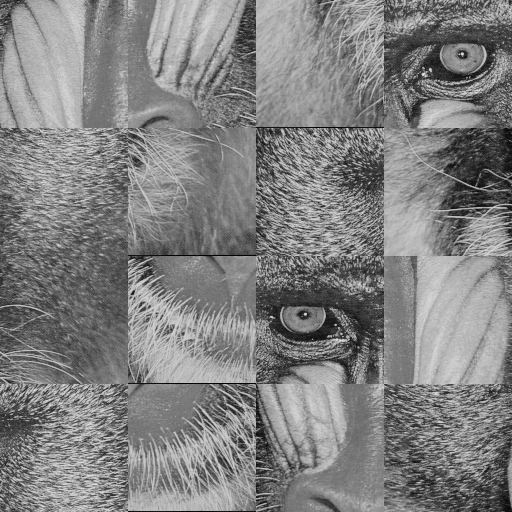
\includegraphics[width=\textwidth,keepaspectratio]{baboon}
                \caption{Imagem original \texttt{baboon}}
                \label{fig:baboon}
            \end{subfigure}
            \begin{subfigure}{0.5\textwidth}
                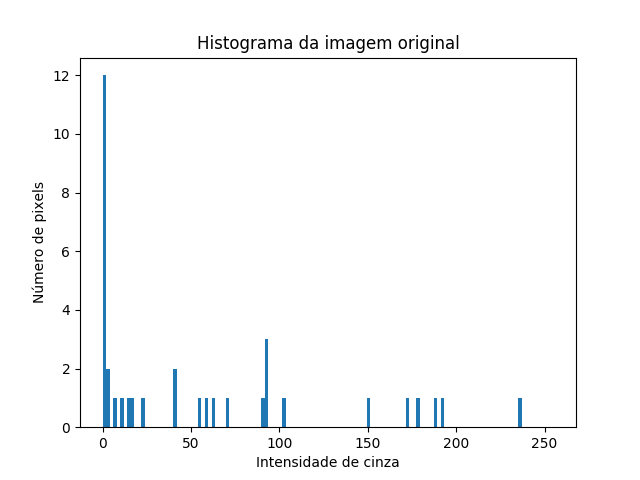
\includegraphics[width=\textwidth,keepaspectratio]{baboon-histograma_in}
                \caption{Histograma da imagem original}
                \label{fig:baboon-histograma}
            \end{subfigure}

            \caption{Características da imagem original de \texttt{baboon}}
        \end{figure}

        Podemos notar na \cref{fig:baboon} que há diversos detalhes finos (como os fios da pelagem, as linhas do nariz e olho). A imagem é em maioria muito nítida e possui bom contraste (\cref{fig:baboon-histograma}).

        Os principais métodos que favorecem as características da imagem, de forma a destacar as linhas e detalhes sem grandes perdas visuais, são os locais: contraste (\cref{fig:baboon-contraste}), Bernsen (\cref{fig:baboon-bernsen}) e média (\cref{fig:baboon-media}).

        Nesses métodos, podemos notar um destaque claro às principais linhas da imagem. Com métodos de realce, talvez seja possível isolar uma imagem ``caricatural'' do babuíno utilizando métodos de eliminação de ruído (mantendo os traços mais grossos).

        Já em Niblack (\cref{fig:baboon-niblack}) e mediana (\cref{fig:baboon-mediana}), há uma proximidade aos mencionados anteriormente, mas as linhas que são destacadas pelos outros nesses métodos não são tão contínuas ou fortes. Isso tornaria a análise proposta (isolar detalhes através de processamento de imagem) mais difícil.

        Nos outros métodos locais SP (\cref{fig:baboon-sp}) e PMS (\cref{fig:baboon-pms}), há muitas perdas pelo nível de brilho ou contraste inadequados à transformação aplicada. Já nos métodos globais global (\cref{fig:baboon-global}) média e mediana aplicados globalmente (cujas imagens não são mostradas por serem muito próximas às do limiar global -- mas podem ser encontradas no repositório do trabalho), não há muito benefício em limiarizar senão para obter uma imagem binária, pois é muito ruidosa e não apresenta qualquer destaque comparado à original.

        \begin{figure}[H]
            \centering
            \begin{subfigure}{0.23\textwidth}
                \includegraphics[width=\textwidth,keepaspectratio]{baboon-final-global}
                \caption{Método global}
                \label{fig:baboon-global}
            \end{subfigure}
            \begin{subfigure}{0.23\textwidth}
                \includegraphics[width=\textwidth,keepaspectratio]{baboon-final-bernsen}
                \caption{Método de Bernsen}
                \label{fig:baboon-bernsen}
            \end{subfigure}
            \begin{subfigure}{0.23\textwidth}
                \includegraphics[width=\textwidth,keepaspectratio]{baboon-final-niblack}
                \caption{Método de Niblack}
                \label{fig:baboon-niblack}
            \end{subfigure}
            \begin{subfigure}{0.23\textwidth}
                \includegraphics[width=\textwidth,keepaspectratio]{baboon-final-sp}
                \caption{Método de SP}
                \label{fig:baboon-sp}
            \end{subfigure}
            \begin{subfigure}{0.23\textwidth}
                \includegraphics[width=\textwidth,keepaspectratio]{baboon-final-pms}
                \caption{Método de PMS}
                \label{fig:baboon-pms}
            \end{subfigure}
            \begin{subfigure}{0.23\textwidth}
                \includegraphics[width=\textwidth,keepaspectratio]{baboon-final-contraste}
                \caption{Método do contraste}
                \label{fig:baboon-contraste}
            \end{subfigure}
            \begin{subfigure}{0.23\textwidth}
                \includegraphics[width=\textwidth,keepaspectratio]{baboon-final-media-local}
                \caption{Método da média local}
                \label{fig:baboon-media}
            \end{subfigure}
            \begin{subfigure}{0.23\textwidth}
                \includegraphics[width=\textwidth,keepaspectratio]{baboon-final-mediana-local}
                \caption{Método da mediana local}
                \label{fig:baboon-mediana}
            \end{subfigure}

            \caption{Comparativo entre diversos métodos de limiarização}
            \label{fig:baboon-limiarizacao}
        \end{figure}

    \subsection{\texttt{Fiducial}}
    \label{sec:fiducial}

        \begin{figure}[h]
            \centering
            \begin{subfigure}{0.30\textwidth}
                \includegraphics[width=\textwidth,keepaspectratio]{fiducial}
                \caption{Imagem original \texttt{fiducial}}
                \label{fig:fiducial}
            \end{subfigure}
            \begin{subfigure}{0.5\textwidth}
                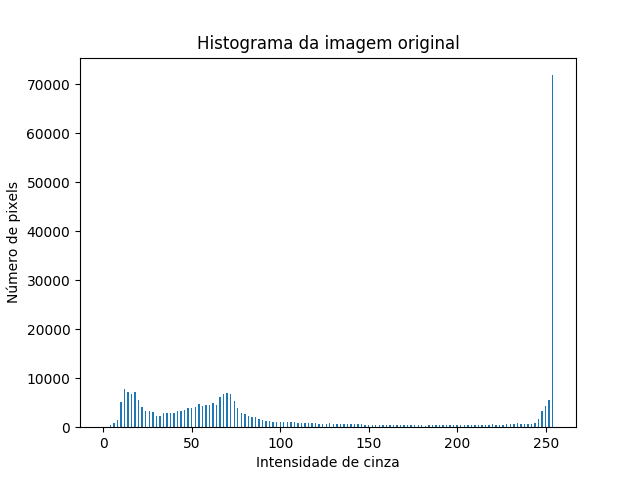
\includegraphics[width=\textwidth,keepaspectratio]{fiducial-histograma_in}
                \caption{Histograma da imagem original}
                \label{fig:fiducial-histograma}
            \end{subfigure}

            \caption{Características da imagem original de \texttt{fiducial}}
        \end{figure}

        Comparando com \texttt{baboon}, que possuía muitos tons de cinza medianos, podemos notar que a \cref{fig:fiducial} é bem diferente: possui poucos tons com maior distribuição.

        Como em \ref{sec:baboon}, os métodos de Bernsen (\cref{fig:fiducial-bernsen}), contraste (\cref{fig:fiducial-contraste}) e média (\cref{fig:fiducial-media}) apresentam ótimos resultados: as formas são bem mantidas e, principalmente em Bernsen, não há muito ruído dentro dos símbolos -- o que seria útil na identificação do recurso. Da mesma forma, o método de PMS (\cref{fig:fiducial-pms}) e os globais (global em \cref{fig:fiducial-global}) possuem pouca utilidade além da original.

        Ao contrário da \cref{sec:baboon}, o método de Niblack (\cref{fig:fiducial-niblack}) e da mediana (\cref{fig:fiducial-mediana}) se afastam dos resultados que consideramos bons: muito ruído é adicionado pela sombra. Por outro lado, SP (\cref{fig:fiducial-sp}) produz um efeito muito bom de destacar silhueta do marcador fiducial e talvez possa ser ajustado para destacar as partes mais claras próximas à luz e escuras, à sombra.


        \begin{figure}[H]
            \centering
            \begin{subfigure}{0.23\textwidth}
                \includegraphics[width=\textwidth,keepaspectratio]{fiducial-final-global}
                \caption{Método global}
                \label{fig:fiducial-global}
            \end{subfigure}
            \begin{subfigure}{0.23\textwidth}
                \includegraphics[width=\textwidth,keepaspectratio]{fiducial-final-bernsen}
                \caption{Método de Bernsen}
                \label{fig:fiducial-bernsen}
            \end{subfigure}
            \begin{subfigure}{0.23\textwidth}
                \includegraphics[width=\textwidth,keepaspectratio]{fiducial-final-niblack}
                \caption{Método de Niblack}
                \label{fig:fiducial-niblack}
            \end{subfigure}
            \begin{subfigure}{0.23\textwidth}
                \includegraphics[width=\textwidth,keepaspectratio]{fiducial-final-sp}
                \caption{Método de SP}
                \label{fig:fiducial-sp}
            \end{subfigure}
            \begin{subfigure}{0.23\textwidth}
                \includegraphics[width=\textwidth,keepaspectratio]{fiducial-final-pms}
                \caption{Método de PMS}
                \label{fig:fiducial-pms}
            \end{subfigure}
            \begin{subfigure}{0.23\textwidth}
                \includegraphics[width=\textwidth,keepaspectratio]{fiducial-final-contraste}
                \caption{Método do contraste}
                \label{fig:fiducial-contraste}
            \end{subfigure}
            \begin{subfigure}{0.23\textwidth}
                \includegraphics[width=\textwidth,keepaspectratio]{fiducial-final-media-local}
                \caption{Método da média local}
                \label{fig:fiducial-media}
            \end{subfigure}
            \begin{subfigure}{0.23\textwidth}
                \includegraphics[width=\textwidth,keepaspectratio]{fiducial-final-mediana-local}
                \caption{Método da mediana local}
                \label{fig:fiducial-mediana}
            \end{subfigure}

            \caption{Comparativo entre diversos métodos de limiarização}
            \label{fig:fiducial-limiarizacao}
        \end{figure}

    \subsection{\texttt{Monarch}}
    \label{sec:monarch}

        \begin{figure}[h]
            \centering
            \begin{subfigure}{0.30\textwidth}
                \includegraphics[width=\textwidth,keepaspectratio]{monarch}
                \caption{Imagem original \texttt{monarch}}
                \label{fig:monarch}
            \end{subfigure}
            \begin{subfigure}{0.5\textwidth}
                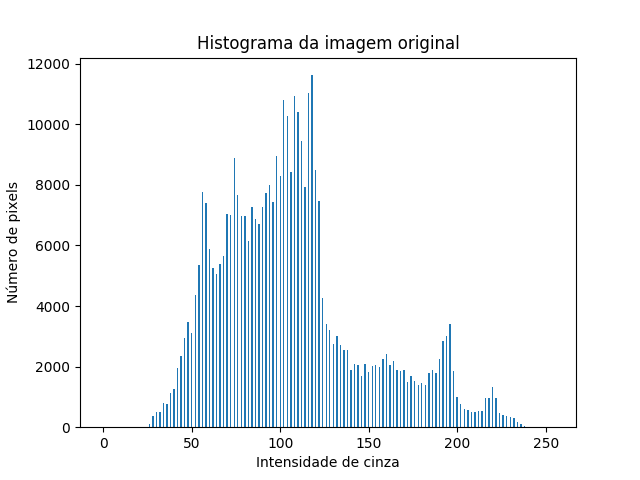
\includegraphics[width=\textwidth,keepaspectratio]{monarch-histograma_in}
                \caption{Histograma da imagem original}
                \label{fig:monarch-histograma}
            \end{subfigure}

            \caption{Características da imagem original de \texttt{monarch}}
        \end{figure}

        Comparando com \texttt{baboon}, que possuía muitos tons de cinza medianos, podemos notar que a \cref{fig:monarch} é bem diferente: possui poucos tons com maior distribuição.

        De novo, temos na \cref{fig:monarch-histograma} um histograma bem diferente dos que já analisamos; o mais próximo é o de \texttt{baboon} (\cref{fig:baboon-histograma}), em que a distribuição é parecida, mas os tons tendem a ser um pouco mais escuros.

        Nessa imagem, há em todos os casos um monte de informação complexa e de difícil interpretação à esquerda (a planta) que só foi possível ignorar no método de SP (\cref{fig:monarch-sp}). Apesar disso, não podemos esperar que esse método sempre isolará o ponto desejado, pois, mesmo que tenha funcionado para \texttt{monarch} e \texttt{fiducial}, não foi o caso em \texttt{baboon}, onde praticamente isolou apenas as partes menos interessantes -- que não foram destacadas pelos outros métodos.

        O método de Bernsen (\cref{fig:monarch-bernsen}), média local (\cref{fig:monarch-media}) e contraste (\cref{fig:monarch-contraste}) foram novamente satisfatórios para isolar linhas contínuas de detalhes interessantes (a borboleta). Comparado com as outras imagens, esses 3 métodos se aproximam bem mais entre si, sendo possível notar apenas a quantidade de ruído existente no fundo, que é menor no da média.

        Novamente, o método de PMS (\cref{fig:monarch-pms}), de Niblack (\cref{fig:monarch-niblack}) e globais (é mostrado apenas o global na \cref{fig:peppers-global}) não produziram resultados de destaque.

        \begin{figure}[H]
            \centering
            \begin{subfigure}{0.23\textwidth}
                \includegraphics[width=\textwidth,keepaspectratio]{monarch-final-global}
                \caption{Método global}
                \label{fig:monarch-global}
            \end{subfigure}
            \begin{subfigure}{0.23\textwidth}
                \includegraphics[width=\textwidth,keepaspectratio]{monarch-final-bernsen}
                \caption{Método de Bernsen}
                \label{fig:monarch-bernsen}
            \end{subfigure}
            \begin{subfigure}{0.23\textwidth}
                \includegraphics[width=\textwidth,keepaspectratio]{monarch-final-niblack}
                \caption{Método de Niblack}
                \label{fig:monarch-niblack}
            \end{subfigure}
            \begin{subfigure}{0.23\textwidth}
                \includegraphics[width=\textwidth,keepaspectratio]{monarch-final-sp}
                \caption{Método de SP}
                \label{fig:monarch-sp}
            \end{subfigure}
            \begin{subfigure}{0.23\textwidth}
                \includegraphics[width=\textwidth,keepaspectratio]{monarch-final-pms}
                \caption{Método de PMS}
                \label{fig:monarch-pms}
            \end{subfigure}
            \begin{subfigure}{0.23\textwidth}
                \includegraphics[width=\textwidth,keepaspectratio]{monarch-final-contraste}
                \caption{Método do contraste}
                \label{fig:monarch-contraste}
            \end{subfigure}
            \begin{subfigure}{0.23\textwidth}
                \includegraphics[width=\textwidth,keepaspectratio]{monarch-final-media-local}
                \caption{Método da média local}
                \label{fig:monarch-media}
            \end{subfigure}
            \begin{subfigure}{0.23\textwidth}
                \includegraphics[width=\textwidth,keepaspectratio]{monarch-final-mediana-local}
                \caption{Método da mediana local}
                \label{fig:monarch-mediana}
            \end{subfigure}

            \caption{Comparativo entre diversos métodos de limiarização}
            \label{fig:monarch-limiarizacao}
        \end{figure}

    \subsection{\texttt{Peppers}}
    \label{sec:peppers}

        \begin{figure}[h]
            \centering
            \begin{subfigure}{0.30\textwidth}
                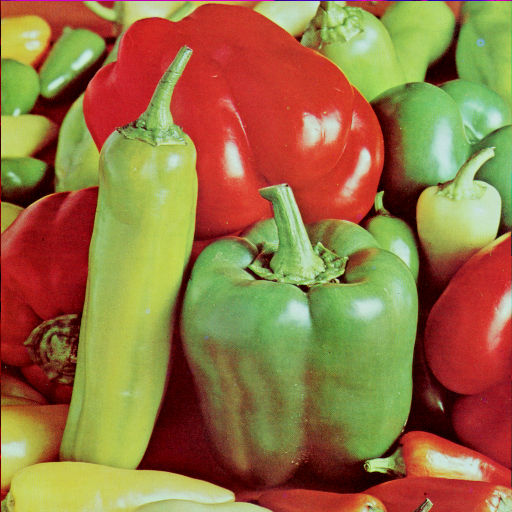
\includegraphics[width=\textwidth,keepaspectratio]{peppers}
                \caption{Imagem original \texttt{peppers}}
                \label{fig:peppers}
            \end{subfigure}
            \begin{subfigure}{0.5\textwidth}
                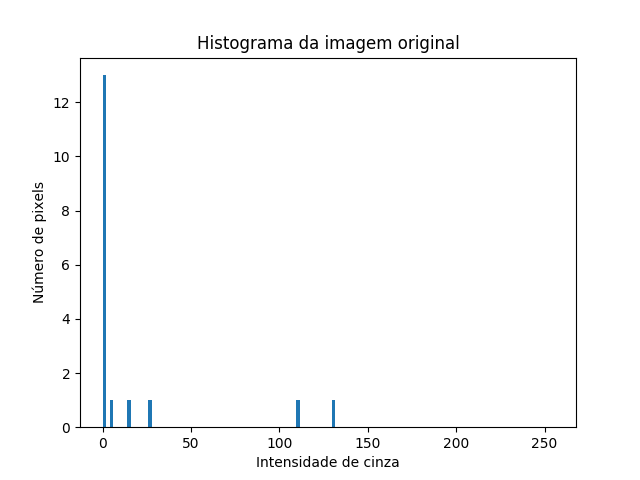
\includegraphics[width=\textwidth,keepaspectratio]{peppers-histograma_in}
                \caption{Histograma da imagem original}
                \label{fig:peppers-histograma}
            \end{subfigure}

            \caption{Características da imagem original de \texttt{peppers}}
        \end{figure}

        Nesta imagem (\cref{fig:peppers}), podemos notar que há poucos pontos claros, predominando tons de cinza. Novamente, os métodos que melhor isolam os objetos (através do destaque às suas silhuetas) foram Bernsen (\cref{fig:peppers-bernsen}), o da média (\cref{fig:peppers-media}) e do contraste (\cref{fig:peppers-contraste}).

        Ao contrário das outras imagens, as diferenças entre esses 3 métodos é maior: o da média sobressai quanto ao tom do ruído em cinza (ruído homogêneo). Também conseguimos reparar que o do contraste se destaca por produzir bordas bastante fortes. O método de Niblack (\cref{fig:peppers-niblack}) dessa vez possui uma característica muito útil: todas as bordas destacadas pelos outros métodos aparecem em cor preta intensa e homogênea (tracejados bem definidos), o que pode ser útil.

        O método de SP (\cref{fig:peppers-sp}) coincide com os resultados anteriores: destaque fino aos tracejados mais fortes. Possui potencial de melhora com ajuste de parâmetros.

        Novamente, PMS (\cref{fig:peppers-pms}) não produziu algo destacável.

        \begin{figure}[H]
            \centering
            \begin{subfigure}{0.23\textwidth}
                \includegraphics[width=\textwidth,keepaspectratio]{peppers-final-global}
                \caption{Método global}
                \label{fig:peppers-global}
            \end{subfigure}
            \begin{subfigure}{0.23\textwidth}
                \includegraphics[width=\textwidth,keepaspectratio]{peppers-final-bernsen}
                \caption{Método de Bernsen}
                \label{fig:peppers-bernsen}
            \end{subfigure}
            \begin{subfigure}{0.23\textwidth}
                \includegraphics[width=\textwidth,keepaspectratio]{peppers-final-niblack}
                \caption{Método de Niblack}
                \label{fig:peppers-niblack}
            \end{subfigure}
            \begin{subfigure}{0.23\textwidth}
                \includegraphics[width=\textwidth,keepaspectratio]{peppers-final-sp}
                \caption{Método de SP}
                \label{fig:peppers-sp}
            \end{subfigure}
            \begin{subfigure}{0.23\textwidth}
                \includegraphics[width=\textwidth,keepaspectratio]{peppers-final-pms}
                \caption{Método de PMS}
                \label{fig:peppers-pms}
            \end{subfigure}
            \begin{subfigure}{0.23\textwidth}
                \includegraphics[width=\textwidth,keepaspectratio]{peppers-final-contraste}
                \caption{Método do contraste}
                \label{fig:peppers-contraste}
            \end{subfigure}
            \begin{subfigure}{0.23\textwidth}
                \includegraphics[width=\textwidth,keepaspectratio]{peppers-final-media-local}
                \caption{Método da média local}
                \label{fig:peppers-media}
            \end{subfigure}
            \begin{subfigure}{0.23\textwidth}
                \includegraphics[width=\textwidth,keepaspectratio]{peppers-final-mediana-local}
                \caption{Método da mediana local}
                \label{fig:peppers-mediana}
            \end{subfigure}

            \caption{Comparativo entre diversos métodos de limiarização}
            \label{fig:peppers-limiarizacao}
        \end{figure}

    \subsection{\texttt{Retina}}
    \label{sec:retina}

        \begin{figure}[h]
            \centering
            \begin{subfigure}{0.30\textwidth}
                \includegraphics[width=\textwidth,keepaspectratio]{retina}
                \caption{Imagem original \texttt{retina}}
                \label{fig:retina}
            \end{subfigure}
            \begin{subfigure}{0.5\textwidth}
                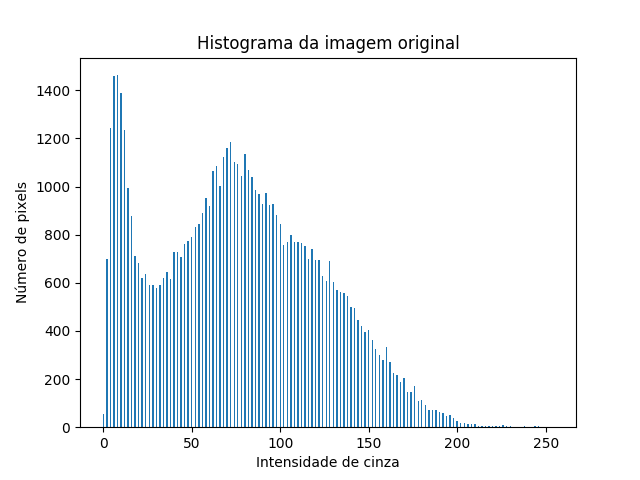
\includegraphics[width=\textwidth,keepaspectratio]{retina-histograma_in}
                \caption{Histograma da imagem original}
                \label{fig:retina-histograma}
            \end{subfigure}

            \caption{Características da imagem original de \texttt{retina}}
        \end{figure}

        A imagem \texttt{retina} (\cref{fig:retina}) possui bem mais tons escuros de acordo com o histograma (\cref{fig:retina-histograma}). Isso, no entanto, não auxilia o método de SP (\cref{fig:retina-sp}) (que destaca áreas bastante escuras), pois há grande quantidade de cinza homogêneo.

        Como nas imagens anteriores, o método de Bernsen (\cref{fig:retina-bernsen}), da média (\cref{fig:retina-media}) e do contraste (\cref{fig:retina-contraste}) produzem os melhores destaques. Porém, o de Niblack (\cref{fig:retina-niblack}) também pode ser destacado como efeito positivo, pois consegue destacar as linhas com um ruído bem mais escuro do que os outros.

        Apesar dessas considerações, o método do contraste dessa vez parece ser o ideal para a situação que é analisar a retina. Isso evidencia novamente que diferentes métodos desempenham de forma diferente no amplo leque de imagens.

        O método de PMS (\cref{fig:retina-pms}) dessa vez mostra os cantos do globo ocular, mas não é de muita utilidade quando comparado aos outros processos.

        \begin{figure}[H]
            \centering
            \begin{subfigure}{0.23\textwidth}
                \includegraphics[width=\textwidth,keepaspectratio]{retina-final-global}
                \caption{Método global}
                \label{fig:retina-global}
            \end{subfigure}
            \begin{subfigure}{0.23\textwidth}
                \includegraphics[width=\textwidth,keepaspectratio]{retina-final-bernsen}
                \caption{Método de Bernsen}
                \label{fig:retina-bernsen}
            \end{subfigure}
            \begin{subfigure}{0.23\textwidth}
                \includegraphics[width=\textwidth,keepaspectratio]{retina-final-niblack}
                \caption{Método de Niblack}
                \label{fig:retina-niblack}
            \end{subfigure}
            \begin{subfigure}{0.23\textwidth}
                \includegraphics[width=\textwidth,keepaspectratio]{retina-final-sp}
                \caption{Método de SP}
                \label{fig:retina-sp}
            \end{subfigure}
            \begin{subfigure}{0.23\textwidth}
                \includegraphics[width=\textwidth,keepaspectratio]{retina-final-pms}
                \caption{Método de PMS}
                \label{fig:retina-pms}
            \end{subfigure}
            \begin{subfigure}{0.23\textwidth}
                \includegraphics[width=\textwidth,keepaspectratio]{retina-final-contraste}
                \caption{Método do contraste}
                \label{fig:retina-contraste}
            \end{subfigure}
            \begin{subfigure}{0.23\textwidth}
                \includegraphics[width=\textwidth,keepaspectratio]{retina-final-media-local}
                \caption{Método da média local}
                \label{fig:retina-media}
            \end{subfigure}
            \begin{subfigure}{0.23\textwidth}
                \includegraphics[width=\textwidth,keepaspectratio]{retina-final-mediana-local}
                \caption{Método da mediana local}
                \label{fig:retina-mediana}
            \end{subfigure}

            \caption{Comparativo entre diversos métodos de limiarização}
            \label{fig:retina-limiarizacao}
        \end{figure}

    \subsection{\texttt{Sonnet}}
    \label{sec:sonnet}

        \begin{figure}[h]
            \centering
            \begin{subfigure}{0.30\textwidth}
                \includegraphics[width=\textwidth,keepaspectratio]{sonnet}
                \caption{Imagem original \texttt{sonnet}}
                \label{fig:sonnet}
            \end{subfigure}
            \begin{subfigure}{0.5\textwidth}
                \includegraphics[width=\textwidth,keepaspectratio]{sonnet-histograma_in}
                \caption{Histograma da imagem original}
                \label{fig:sonnet-histograma}
            \end{subfigure}

            \caption{Características da imagem original de \texttt{sonnet}}
        \end{figure}

        Nessa análise da \cref{fig:sonnet} com texto \texttt{sonnet} sob ruim iluminação (não é uniforme e é fraca na maioria da imagem) com foco não ideal, temos um problema muito prático que é o isolamento de letras para melhorar sua visualização.

        Nesses casos, a maioria dos métodos introduz muitos ruídos que tornam muito difícil a interpretação do que está escrito nessa imagem de relativamente pequena dimensão. Ou seja, é uma correção difícil. De fato isso é confirmado pelas imagens da \cref{fig:sonnet-limiarizacao}: mesmo aproximando a imagem em visualizadores, não é fácil decifrar alguns caracteres.

        Nessa imagem podemos notar que Bernsen (\cref{fig:sonnet-bernsen}) apresenta artefatos verticais, tornando vários dos caracteres ilegíveis assim como o da média (\cref{fig:sonnet-media}), que foram avaliados muito bem em outras imagens. Com isso, o da mediana (\cref{fig:sonnet-mediana}) -- que possui menos ruído em toda imagem, principalmente entre as letras -- e do contraste (\cref{fig:sonnet-contraste}) se destacam; não por tornar o texto legível, mas apenas por manter o formato das letras.

        Os métodos de Niblack (\cref{fig:sonnet-niblack}), de PMS (\cref{fig:sonnet-pms}) e de SP (\cref{fig:sonnet-sp}) não produzem informação útil com os parâmetros padrões sugeridos, assim como os globais.

        \begin{figure}[H]
            \centering
            \begin{subfigure}{0.20\textwidth}
                \includegraphics[width=\textwidth,keepaspectratio]{sonnet-final-global}
                \caption{Método global}
                \label{fig:sonnet-global}
            \end{subfigure}
            \begin{subfigure}{0.20\textwidth}
                \includegraphics[width=\textwidth,keepaspectratio]{sonnet-final-bernsen}
                \caption{Método de Bernsen}
                \label{fig:sonnet-bernsen}
            \end{subfigure}
            \begin{subfigure}{0.20\textwidth}
                \includegraphics[width=\textwidth,keepaspectratio]{sonnet-final-niblack}
                \caption{Método de Niblack}
                \label{fig:sonnet-niblack}
            \end{subfigure}
            \begin{subfigure}{0.20\textwidth}
                \includegraphics[width=\textwidth,keepaspectratio]{sonnet-final-sp}
                \caption{Método de SP}
                \label{fig:sonnet-sp}
            \end{subfigure}
            \begin{subfigure}{0.20\textwidth}
                \includegraphics[width=\textwidth,keepaspectratio]{sonnet-final-pms}
                \caption{Método de PMS}
                \label{fig:sonnet-pms}
            \end{subfigure}
            \begin{subfigure}{0.20\textwidth}
                \includegraphics[width=\textwidth,keepaspectratio]{sonnet-final-contraste}
                \caption{Método do contraste}
                \label{fig:sonnet-contraste}
            \end{subfigure}
            \begin{subfigure}{0.20\textwidth}
                \includegraphics[width=\textwidth,keepaspectratio]{sonnet-final-media-local}
                \caption{Método da média local}
                \label{fig:sonnet-media}
            \end{subfigure}
            \begin{subfigure}{0.20\textwidth}
                \includegraphics[width=\textwidth,keepaspectratio]{sonnet-final-mediana-local}
                \caption{Método da mediana local}
                \label{fig:sonnet-mediana}
            \end{subfigure}

            \caption{Comparativo entre diversos métodos de limiarização}
            \label{fig:sonnet-limiarizacao}
        \end{figure}

    \subsection{\texttt{Wedge}}
    \label{sec:wedge}

        \begin{figure}[h]
            \centering
            \begin{subfigure}{0.30\textwidth}
                \includegraphics[width=\textwidth,keepaspectratio]{wedge}
                \caption{Imagem original \texttt{wedge}}
                \label{fig:wedge}
            \end{subfigure}
            \begin{subfigure}{0.5\textwidth}
                \includegraphics[width=\textwidth,keepaspectratio]{wedge-histograma_in}
                \caption{Histograma da imagem original}
                \label{fig:wedge-histograma}
            \end{subfigure}

            \caption{Características da imagem original de \texttt{wedge}}
        \end{figure}

        A imagem é um bom exemplo do que uma indústria poderia utilizar com uma câmera de análise ``top down''. O histograma da \cref{fig:wedge-histograma} mostra que a imagem pode estar muito iluminada pelo fundo que possui alta reflexibilidade, o que ainda não atrapalha os melhores métodos Bernsen (\cref{fig:wedge-bernsen}), contraste (\cref{fig:wedge-contraste}) e média (\cref{fig:wedge-media}) (com exceção do da mediana -- \cref{fig:wedge-mediana} --, mas este já não foi capaz de identificar a borda com precisão).

        O método de Niblack (\cref{fig:wedge-niblack}) mostra com muito destaque as bordas do objeto, porém erra à direita, por conta da sombra, que não atrapalham o de Bernsen, o da média e o do contraste. Para melhorar a visualização da borda, o método da média local parece ser ideal pois a sombra confunde-se mais com o ruído.

        Como na \cref{sec:sonnet}, o método de PMS (\cref{fig:wedge-pms}) e global (\cref{fig:wedge-global}) foram de pouco proveito.

        \begin{figure}[H]
            \centering
            \begin{subfigure}{0.23\textwidth}
                \includegraphics[width=\textwidth,keepaspectratio]{wedge-final-global}
                \caption{Método global}
                \label{fig:wedge-global}
            \end{subfigure}
            \begin{subfigure}{0.23\textwidth}
                \includegraphics[width=\textwidth,keepaspectratio]{wedge-final-bernsen}
                \caption{Método de Bernsen}
                \label{fig:wedge-bernsen}
            \end{subfigure}
            \begin{subfigure}{0.23\textwidth}
                \includegraphics[width=\textwidth,keepaspectratio]{wedge-final-niblack}
                \caption{Método de Niblack}
                \label{fig:wedge-niblack}
            \end{subfigure}
            \begin{subfigure}{0.23\textwidth}
                \includegraphics[width=\textwidth,keepaspectratio]{wedge-final-sp}
                \caption{Método de SP}
                \label{fig:wedge-sp}
            \end{subfigure}
            \begin{subfigure}{0.23\textwidth}
                \includegraphics[width=\textwidth,keepaspectratio]{wedge-final-pms}
                \caption{Método de PMS}
                \label{fig:wedge-pms}
            \end{subfigure}
            \begin{subfigure}{0.23\textwidth}
                \includegraphics[width=\textwidth,keepaspectratio]{wedge-final-contraste}
                \caption{Método do contraste}
                \label{fig:wedge-contraste}
            \end{subfigure}
            \begin{subfigure}{0.23\textwidth}
                \includegraphics[width=\textwidth,keepaspectratio]{wedge-final-media-local}
                \caption{Método da média local}
                \label{fig:wedge-media}
            \end{subfigure}
            \begin{subfigure}{0.23\textwidth}
                \includegraphics[width=\textwidth,keepaspectratio]{wedge-final-mediana-local}
                \caption{Método da mediana local}
                \label{fig:wedge-mediana}
            \end{subfigure}

            \caption{Comparativo entre diversos métodos de limiarização}
            \label{fig:wedge-limiarizacao}
        \end{figure}


\section{Conclusão}

    De todos os métodos analisados, considerando como parâmetro de avaliação a possibilidade de isolar e reconhecer partes interessantes da imagem, por exemplo, silhuetas, linhas contínuas e talvez até formatos, os que melhor desempenharam foram o da média e o de Bernsen, possuindo menos ruídos que o do contraste (possui as mesmas características). Também é importante mencionar o método de SP, que conseguiu separar muito bem em várias imagens apenas os detalhes mais escuros, deixando silhuetas bem destacadas.

    De forma geral, é necessário avaliar em cada aplicação o melhor método. Apesar de ser evidente que a limiarização pode auxiliar no destaque de bordas, não há um método útil a todo tipo de imagem.

    Do aspecto de uso prático, a imagem da borboleta \texttt{monarch} foi a mais poluída e de dificil isolamento, enquanto os resultados em \texttt{fiducial} e \texttt{sonnet} foram bastante satisfatórios considerando a luminosidade não uniforme. Em todos os casos, houve pouco proveito dos métodos globais (limiarização global utilizando uma constante, a média ou ainda a mediana da imagem toda) pois ignorava grandes trechos da imagem ou produzia muito ruído próximo das cores medianas.

    Talvez seja possível com um controle sutil dos parâmetros melhorar o método de SP e ainda corrigir o de PMS, que, inclusive nas imagens de baixo contraste, não produziu algo de destaque. Também podemos considerar aprimorar através de parâmetros ou outros realces o filtro de Niblack, que produz traços fortes contínuos pretos entre ruídos escuros, o que é algo difícil de isolar.

\end{document}
